\section{Introduction and motivation}
\label{1}
The last decade has seen a remarkable resurgence in attention towards space exploration. After several years of decay from the heights of the moon missions, the renewed interest from governmental bodies and private companies, the technological advancements in material science and reusable rockets, and the reemergence of human spaceflight have generated a positive feedback loop that has directed major investments into the sector.

Many groundbreaking endeavours have emerged: the rise of private space companies, led by industry giants such as Elon Musk's SpaceX and Jeff Bezos' Blue Origin, has democratized and made more accessible the space sector. Revolutionary new launchers, such as the fully reusable Falcon and the super heavy Starship (with the latter recently undergoing its first test flight), have axed the cost barrier for launching payload into space, opening up unprecedented opportunities for scientific research, commercial ventures, and space exploration.

Many national and international space agencies have also demonstrated a significant increase in interest. Among various mission of the European Space Agency (ESA), the following are noteworthy:

\begin{itemize}
    \item JUICE (launched on 14 April 2023): tasked with the exploration of Jupiter's icy moons (Europa, Ganymede and Callisto), housing a magnetometer made by Imperial College.
    \item ExoMars (initially scheduled for the second half of 2023, but currently postponed to 2028): ESA's astrobiology mission designated to investigate signs of past life on the red planet.
    \item Hera (scheduled to launch in October 2024): a mission towards the Didymos binary asteroid system tasked with examining the aftermath of a the collision between the aforementioned asteroid and DART (a previous NASA mission which investigated a method of planetary defense against near-Earth objects).
\end{itemize}

On the other side of the ocean, NASA has been engaged with building and launching the Webb space telescope.  Currently stationed at the sun-earth L2 Lagrange point, it is expected to make groundbreaking discoveries thanks to its infrared camera, which will allow to see objects too distant or faint to be captured by earth-stationed telescopes or the Hubble telescope.

Meanwhile, NASA's Artemis program (in collaboration with ESA and JAXA) plans to establish a long-term human presence on the moon, through the construction of a permanent outpost on the lunar surface. An extraterrestrial space station, called Gateway, will also be built. It will be placed into lunar orbit and will serve as a communication hub and temporary habitation module for astronauts in deep space missions.

The increased interest in space exploration has led to the need to efficiently launch and land greater and greater payloads has emerged. While progress on the former objective has been very good (thanks, for example, to reusable rockets such as the aforementioned Falcon and Starship, or the more conventional Space Launch System), advancements in the latter area are still lacking.

\subsection{Entry, descent and landing}
Getting a spacecraft to safely land onto the surface of a planet is a complex undertaking, characterised by significant challenges \cite{aerothermonotes}. It is composed by three parts: 
\begin{itemize}
    \item Entry, during which the spacecraft transitions from outer space into the planet's atmosphere (and hence reduces its velocity by several orders of magnitude).
    \item Descent, which starts after the spacecraft reaches its terminal velocity.
    \item Landing, the final stage during which the spacecraft is gently brought to a standstill on the planetary surface.
\end{itemize}

Among the three, atmospheric entry is the stage which poses the most threats to the vehicle's safety. Since the interplanetary transfer velocity is usually of the order of several \si{\km\per\s}, and the most common mechanism for achieving descent is to deploy subsonic parachutes (which require the velocity magnitude not to exceed 200 to 300 \si{\m\per\s}), a vast amount of kinetic energy has to be dissipated. 

Historically, the most common and cost-effective approach to achieve atmospheric entry has been to employ aerobraking, which consists in relying on  friction with the planet atmosphere to slow the spacecraft down. This method, while being significantly less expensive than others (such as using retropropulsion), poses the challenge of having to halt heat from leaking into the very sensible payload. Minimising the heat transfer to the body is thus of the utmost importance.

Peak heat transfer rate $\dot{q}_{\max }$ and total heat load $Q$ are determined by \autoref{eq:peakheat} and \autoref{eq:totalheat} respectively
\begin{equation}
    \dot{q}_{\max } \propto \sqrt{B C \sin (FPA)}
    \label{eq:peakheat}
\end{equation}
\begin{equation}
    Q \propto \sqrt{\frac{B C}{\sin (FPA)}}
    \label{eq:totalheat}
\end{equation}
in which $BC$ is the ballistic coefficient and $FPA$ is the flight path angle.
Hence, both peak heating rate and the total heating on the spacecraft are proportional to the ballistic coefficient. Thus minimising BC is essential. 

The ballistic coefficient can be conceptualised as a measure of the ability of a body to counteract air resistance, and is calculated as in \autoref{eq:balcof}, where $BC$ is the ballistic coefficient, $m$ is the spacecraft mass, $C_D$ is the spacecraft coefficient of drag and $A$ is the aeroshell incident surface area.
\begin{equation}
    B C=\frac{m}{C_D A}
    \label{eq:balcof}
\end{equation}
Conventionally, this has been done by increasing the vehicle frontal area. However, with the increased payloads required by future missions, this will no longer be achievable, as the aeroshell size will be limited by the launcher payload fairing diameter. New techniques have thus emerged to tackle this problem.

\subsection{Future of EDL}
To overcome the limit of the launcher fairing size, three new aeroshell technologies have emerged:
\begin{itemize}
    \item Mechanically deployable aeroshells, which elude the fairing size limitation by stowing the heat shield and deploying it only after separating from the payload housing \cite{aerothermonotes}. Examples where this concept has been applied include ADEPT from NASA \cite{adeptfeasibility} (which has already undergone extensive testing \cite{adepttest}) and IRENE, from the Italian Space Agency (ASI) \cite{irene}.
    \item Inflatable aeroshells (such as the HIAD concept from NASA \cite{hiad}), which employ the same concept, but deploy the aeroshell by inflating it rather than mechanically expanding it. 
    \item Rigid, mid $L/D$ aeroshells, which consist in a static fuselage-type shape which decreases $BC$ by flying a lifting path \cite{aerothermonotes, midld}
\end{itemize}

Due to their complex nature, deployable aeroshells present a fascinating set of challenges. These problems encompass structural intricacies, such as the increased failure likelihood originating from the deployment or the interlocking of the ribs for mechanically deployable ones, as well as material science complexities, such as the need of a heat shield material able to fold. Furthermore, the more sophisticated geometry makes the aerothermodynamic analysis significantly more challenging.

\subsection{HATHOR}

Imperial College London has also developed its own implementation of a mechanically deployable aeroshell, named HATHOR \cite{hathordesign}, which can be seen in \autoref{fig:hathorsketch}. It features an \SI{2.65}{\m}, 8 rib aluminium design with a \SI{70}{\deg} half cone deployed angle (which reduces to \SI{20}{\deg} when stowed) \cite{hathordesign} and a \SI{14}{\mm} thick ablative TPS made from SLA-561 V \cite{hathoraero1}. HATHOR has undergone structural \cite{hathordesign} and aerothermal analysis \cite{hathoraero1}, and full scale mechanical testing \cite{hathorstructest}.

\begin{figure}[ht]
    \centering
    \begin{subfigure}{0.43\textwidth}
        \centering
        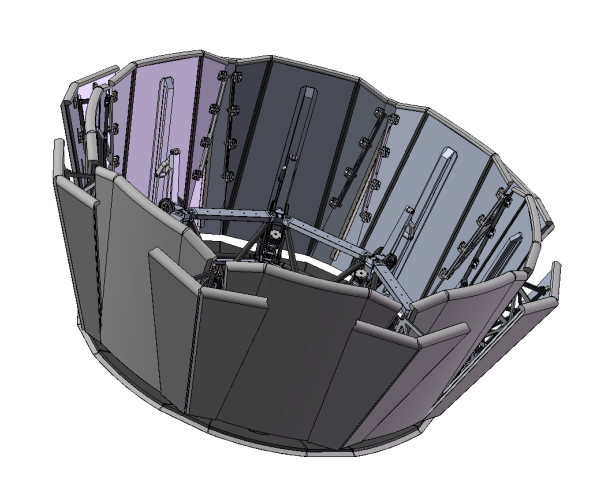
\includegraphics[width=\textwidth]{../Images/1. Introduction/HathorStowed.png}
        \caption{Deployed configuration.}
    \end{subfigure}
    \hfill
    \begin{subfigure}{0.56\textwidth}
        \centering
        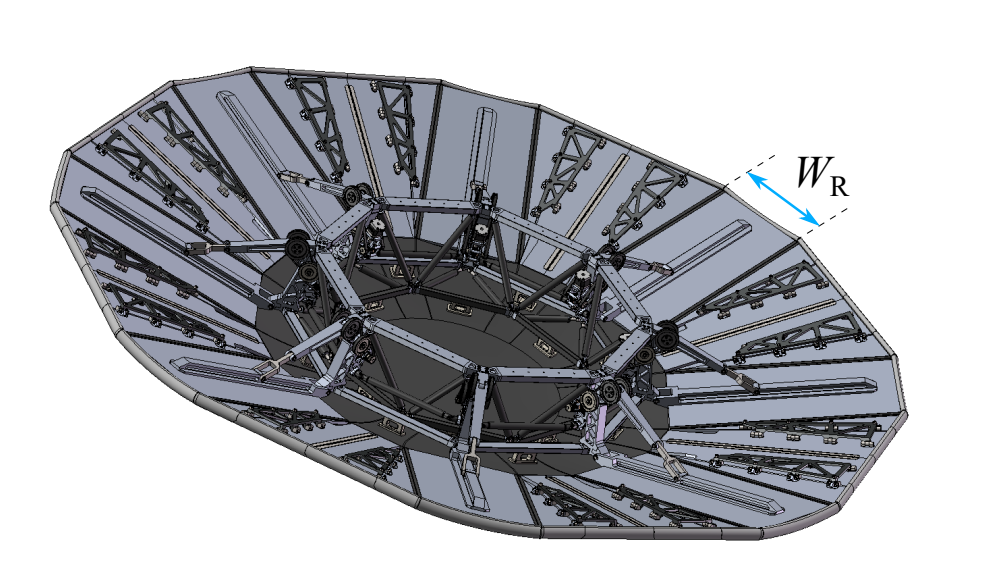
\includegraphics[width=\textwidth]{../Images/1. Introduction/HathorDeployed.png}  
        \caption{Stowed configuration.}
    \end{subfigure}
    \caption{Sketches of HATHOR \cite{hathoraero1}.}
    \label{fig:hathorsketch}
\end{figure}

This aerothermal analysis was conducted using both HEAT-3D \cite{heat3d}, a reduced order model for rapid prototyping of thermal protection systems \cite{hathoraero1}, and wind tunnel experiment paired with a coupled heat transfer CFD simulation \cite{hathoraero2}. 
In the latter, notable discrepancies emerged between the physical experiment and the simulation. These discrepancies sparked a discussion, which highlighted the possibility that they might be caused by rarefied flow, a condition known to impact aerodynamic properties. 

The combination of this intriguing intuitions and their relevance in the aforementioned situation of heightened interest into space exploration served as the primary motivation behind the research presented in this thesis. The foucs of this study revolves around exploring heat transfer in simple bodies under hypersonic rarefied conditions, particularly focusing on sharp corners, with the aims of investigating the evolution of Stanton number in rarefied flow and determining a correction factor to be used in codes for rapid aerothermal prototyping, such as HEAT-3D.

In \autoref{section:2} the theoretical background behind rarefied flow will be investigated and relevant research about its modelling will be presented.

Section \ref{section:3} will outline the general principles of operations of a Direct Simulation Monte Carlo code, which will subsequently be used to design and validate four set of simulations: varying global Knudsen number, varying edge radius, constant local Knudsen number and varying angle of attack. a full set of convergence studies will also be conducted, in order to ensure the accuracy of the simulatons.

The main findings of the research will thus be outlined and discussed in \autoref{section:4}.

